
% Terceiro capítulo deste trabalho.
%--------------------------------------
\chapter{Ferramentas e Tecnologias}

Neste capítulo serão apresentadas as ferramentas e tecnologias utilizadas ao longo do desenvol-vimento do projeto. Serão abordadas as tecnologias utilizadas para o desenvolvimento do \textit{back-end} e do \textit{front-end}, bem como as ferramentas de apoio ao desenvolvimento e gestão do projeto.

\section{Visual Studio Code}
    
    \subsection{O que é o Visual Studio Code?}
        O Visual Studio Code (VS Code) é um editor de código de código aberto desenvolvido pela Microsoft, o qual tem como algumas funcionalidades:
        \begin{itemize}
            \item Edição de código com suporte a várias linguagens de programação;
            \item Terminal de comandos integrado;
            \item Controlo de Versões;
        \end{itemize}
        \begin{figure}[h]
            \centering
            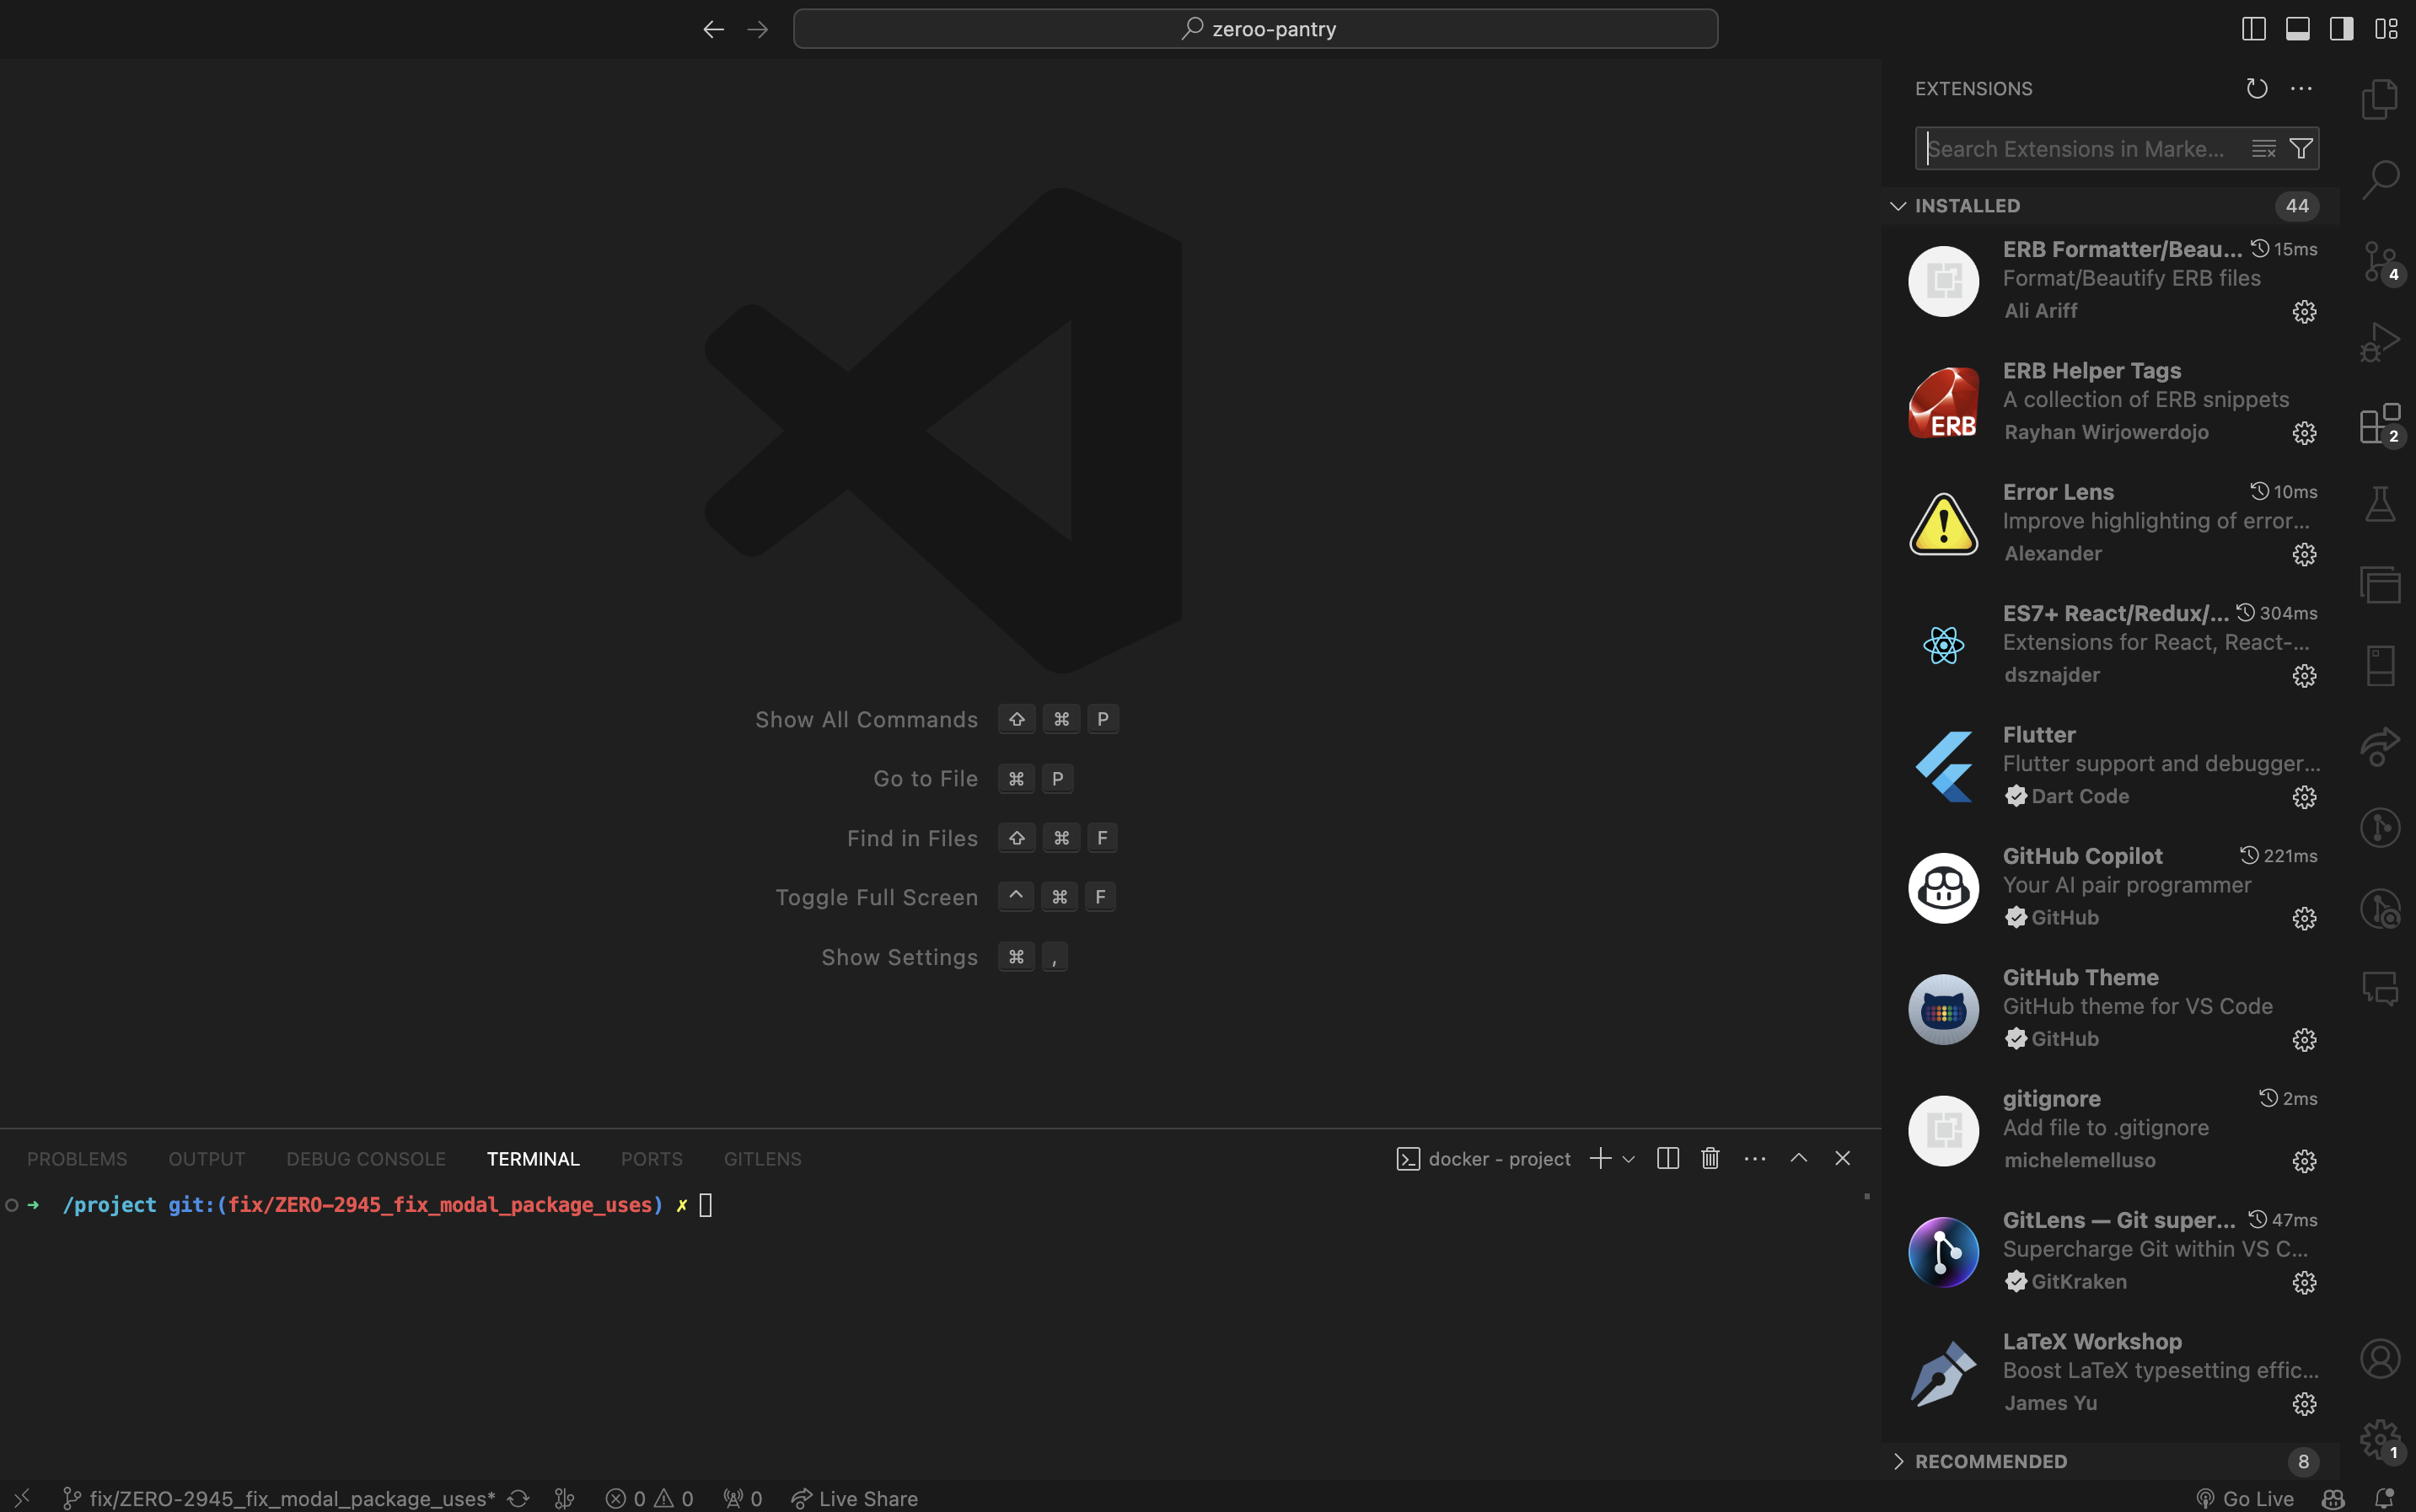
\includegraphics[width=1\textwidth]{Imagens/visual_studio_code.png} % Use your image file name and path
            \caption{Interface do Visual Studio Code}
            \label{fig:vscode}
        \end{figure}

    \newpage
    \subsection{Extensões}
        No início do estágio, foram instaladas algumas extensões no Visual Studio Code, de forma a facilitar o desenvolvimento do projeto e formatação do códgio. Algumas das extensões instaladas foram:
        \begin{itemize}[noitemsep, topsep=0pt]
            \item \textbf{Solargprah:} Ferramenta que proporciona intellisense \textit{features} através do \textit{language server protocol} da Microsoft;
            \item \textbf{Rails DB Schema:} Ferramenta que fornece definições e conclusões para \textit{Rails DB Schemas};
            \item \textbf{Git Lens:} GitLens é a ferramenta projetada para melhorar o foco, a produtividade e a colaboração com um poderoso conjunto de ferramentas para a equipa a enten-der, escrever e rever melhor o código;
            \item \textbf{Gitignore:} Ferramenta que oferece uma maior facilidade em adicionar ficheiros ao \textit{.gitignore};
            \item \textbf{ERB Helper:} Conjunto de \textit{snnipets} do VS Code para código \textit{ERB};
            \item \textbf{End wise:} Esta é uma extensão que adiciona a \textit{keyword} "end" às estruturas de código em linguagens como Ruby ou Crystal, mantendo os níveis de indentação corretos;
            \item \textbf{Auto rename tag:} Ferramenta utilizada para quando uma tag é renomeada, a tag de abertura/fecho complementar é renomeada sozinha para corresponder ao novo nome da tag;
        \end{itemize}

\section{Docker}
\section{Microsoft Teams}
\section{Clickup}
\section{Git}
\section{GitLab}
\section{Ruby on Rails}
\section{Hotwire}
\section{Turbo Frames}
\section{Turbo Streams}
\section{Stimulus}